\chapter{Valores experimentales} \label{implementacion}

\section{Backpropagation}
\begin{figure}[H]
    \centering
    \begin{subfigure}[H]{0.45\textwidth}
    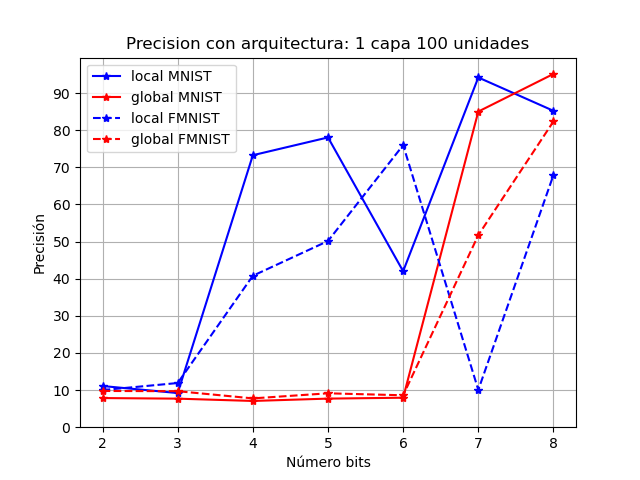
\includegraphics[width=\textwidth]{imagenes/backprop/Precision con arquitectura: 1 capa 100 unidades.png}
    \end{subfigure}
    \begin{subfigure}[H]{0.45\textwidth}
    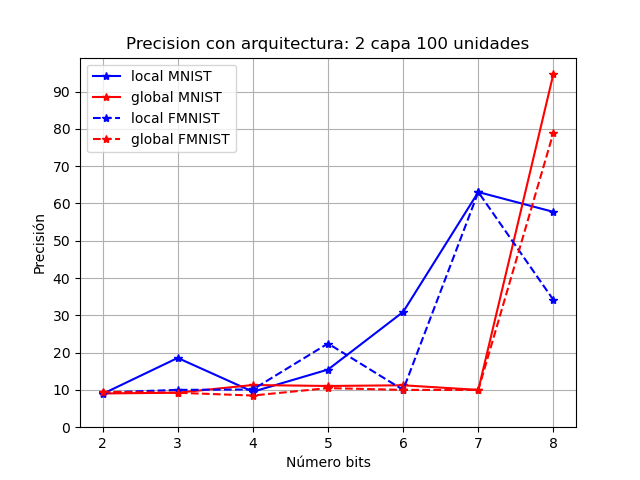
\includegraphics[width=\textwidth]{imagenes/backprop/Precision con arquitectura: 2 capa 100 unidades.png}
    \end{subfigure}
    \begin{subfigure}[H]{0.45\textwidth}
    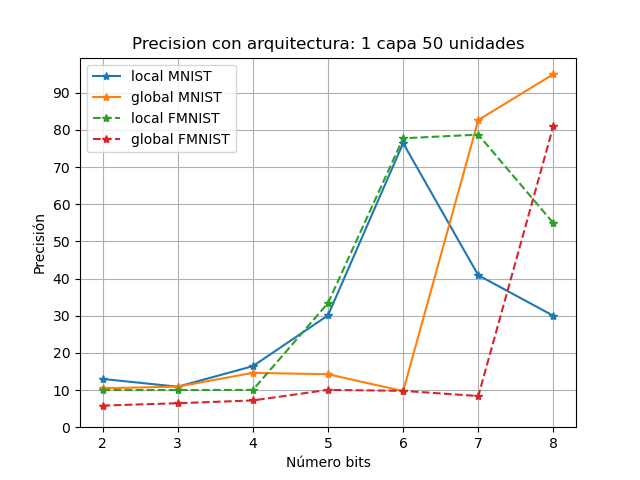
\includegraphics[width=\textwidth]{imagenes/backprop/Precision con arquitectura: 1 capa 50 unidades.png}
    \end{subfigure}
    \begin{subfigure}[H]{0.45\textwidth}
    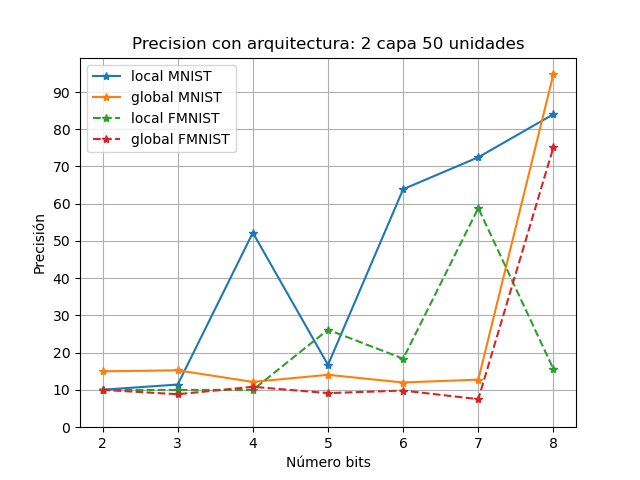
\includegraphics[width=\textwidth]{imagenes/backprop/Precision con arquitectura: 2 capa 50 unidades.png}
    \end{subfigure}
    \begin{subfigure}[H]{0.45\textwidth}
    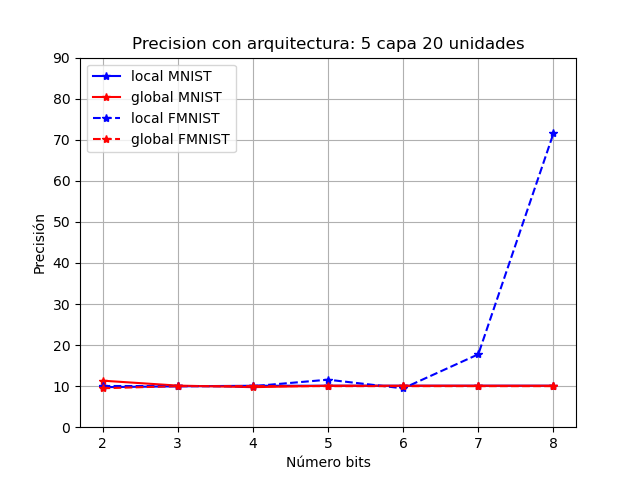
\includegraphics[width=\textwidth]{imagenes/backprop/Precision con arquitectura: 5 capa 20 unidades.png} 
    \end{subfigure}
\end{figure}
\newpage
\section{HSIC}
\begin{figure}[H]
    \centering
    \begin{subfigure}[H]{0.45\textwidth}
    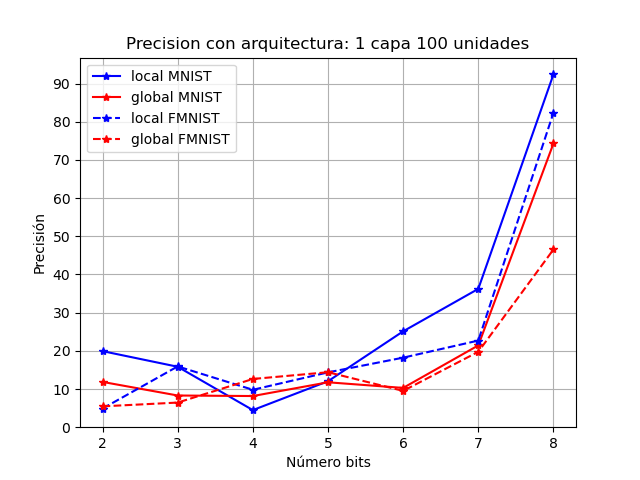
\includegraphics[width=\textwidth]{imagenes/HSIC/Precision con arquitectura: 1 capa 100 unidades.png}
    \end{subfigure}
    \begin{subfigure}[H]{0.45\textwidth}
    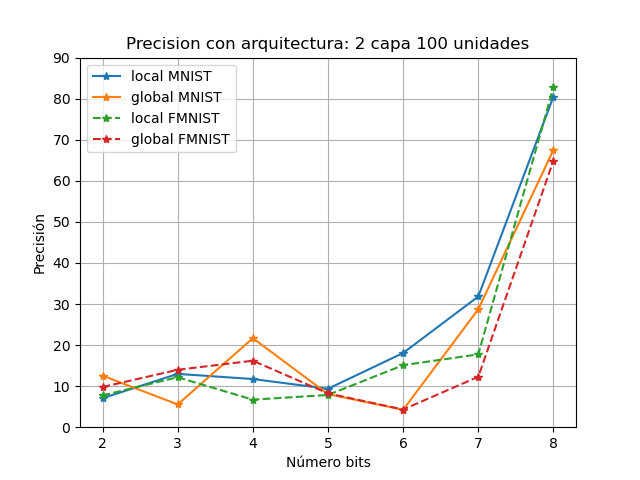
\includegraphics[width=\textwidth]{imagenes/HSIC/Precision con arquitectura: 2 capa 100 unidades.png}
    \end{subfigure}
    \begin{subfigure}[H]{0.45\textwidth}
    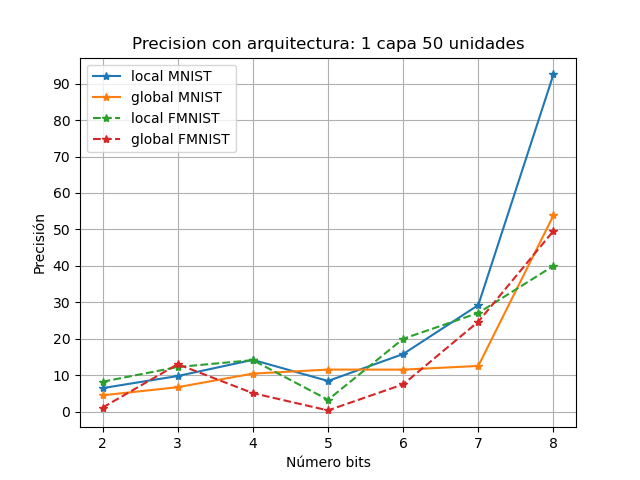
\includegraphics[width=\textwidth]{imagenes/HSIC/Precision con arquitectura: 1 capa 50 unidades.png}
    \end{subfigure}
    \begin{subfigure}[H]{0.45\textwidth}
    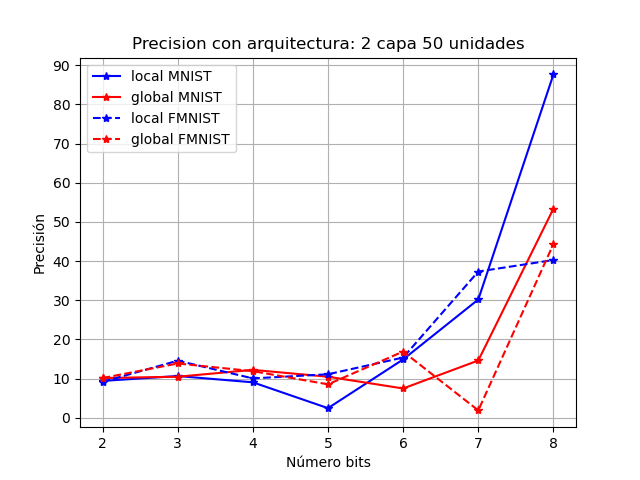
\includegraphics[width=\textwidth]{imagenes/HSIC/Precision con arquitectura: 2 capa 50 unidades.png}
    \end{subfigure}
    \begin{subfigure}[H]{0.45\textwidth}
    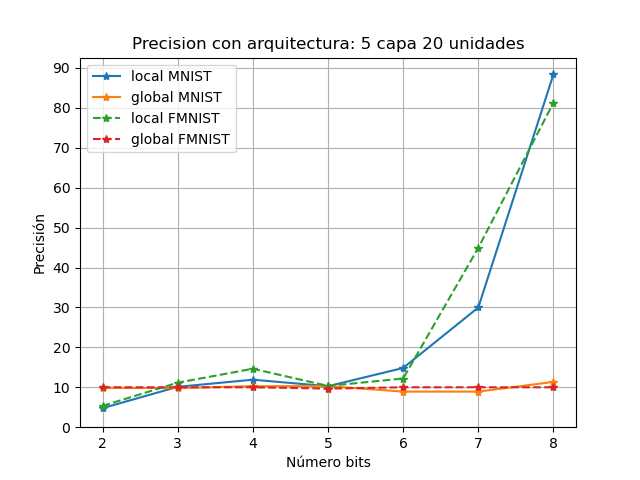
\includegraphics[width=\textwidth]{imagenes/HSIC/Precision con arquitectura: 5 capa 20 unidades.png} 
    \end{subfigure}
\end{figure}

\section{FeedbackAlignment}
\begin{figure}[H]
    \centering
    \begin{subfigure}[H]{0.45\textwidth}
    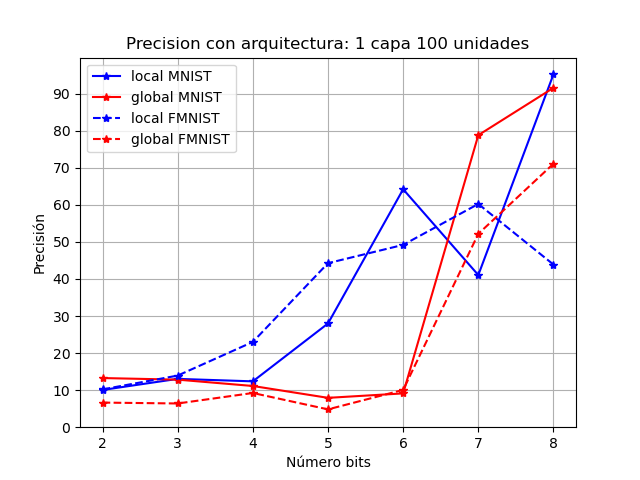
\includegraphics[width=\textwidth]{imagenes/fa/Precision con arquitectura: 1 capa 100 unidades.png}
    \end{subfigure}
    \begin{subfigure}[H]{0.45\textwidth}
    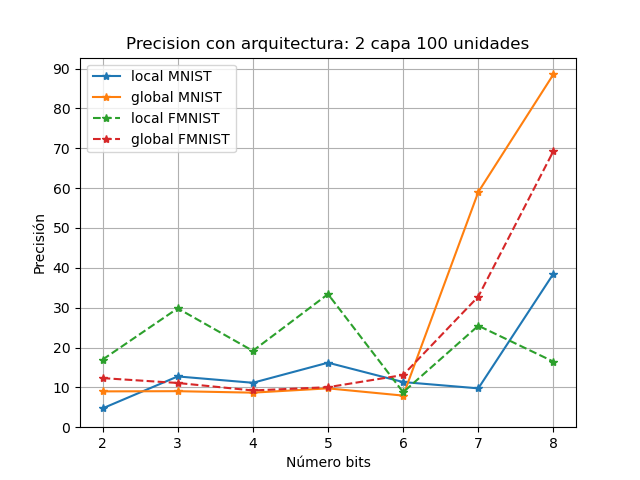
\includegraphics[width=\textwidth]{imagenes/fa/Precision con arquitectura: 2 capa 100 unidades.png}
    \end{subfigure}
    \begin{subfigure}[H]{0.45\textwidth}
    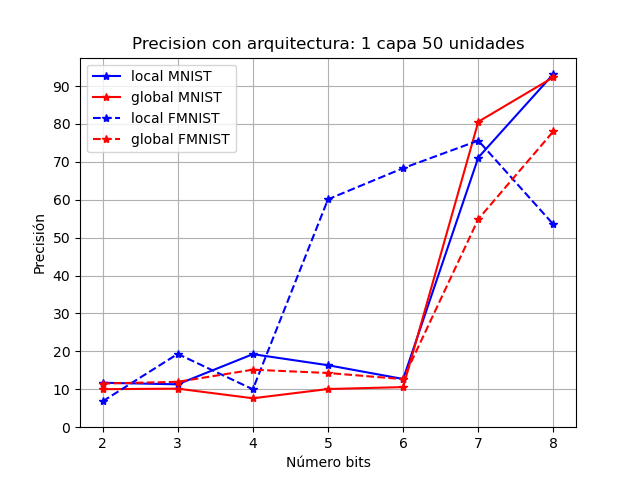
\includegraphics[width=\textwidth]{imagenes/fa/Precision con arquitectura: 1 capa 50 unidades.png}
    \end{subfigure}
    \begin{subfigure}[H]{0.45\textwidth}
    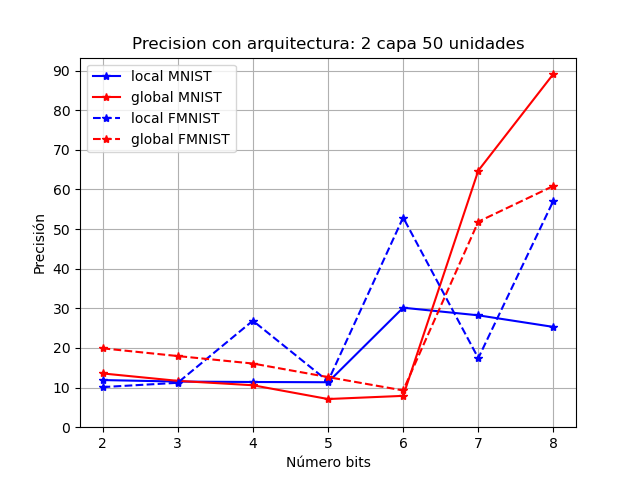
\includegraphics[width=\textwidth]{imagenes/fa/Precision con arquitectura: 2 capa 50 unidades.png}
    \end{subfigure}
    \begin{subfigure}[H]{0.45\textwidth}
    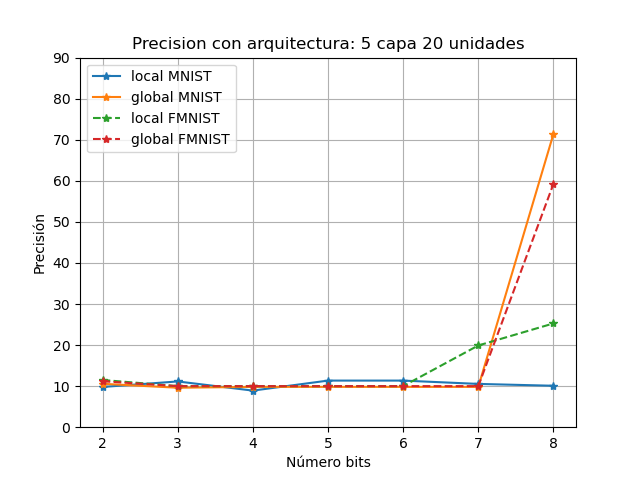
\includegraphics[width=\textwidth]{imagenes/fa/Precision con arquitectura: 5 capa 20 unidades.png} 
    \end{subfigure}
\end{figure}

\section{Synthetic gradients}
\begin{figure}[H]
    \centering
    \begin{subfigure}[H]{0.45\textwidth}
    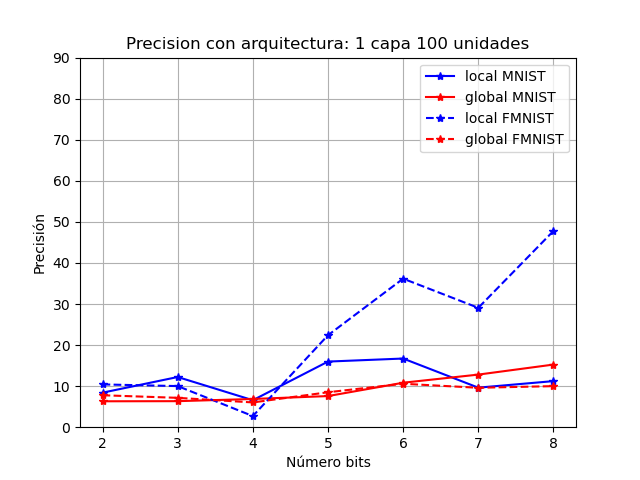
\includegraphics[width=\textwidth]{imagenes/dni/Precision con arquitectura: 1 capa 100 unidades.png}
    \end{subfigure}
    \begin{subfigure}[H]{0.45\textwidth}
    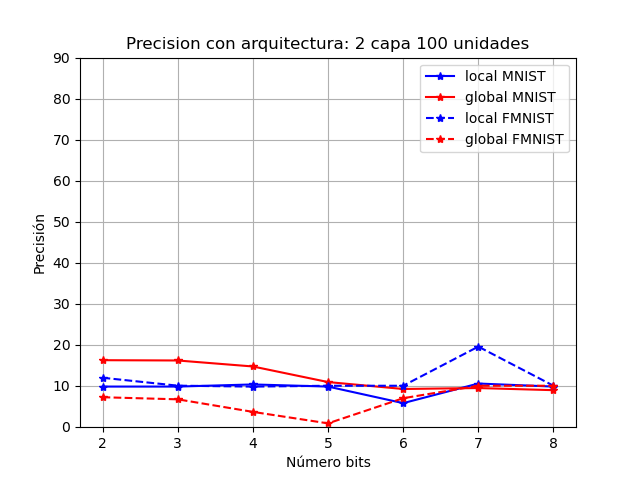
\includegraphics[width=\textwidth]{imagenes/dni/Precision con arquitectura: 2 capa 100 unidades.png}
    \end{subfigure}
    \begin{subfigure}[H]{0.45\textwidth}
    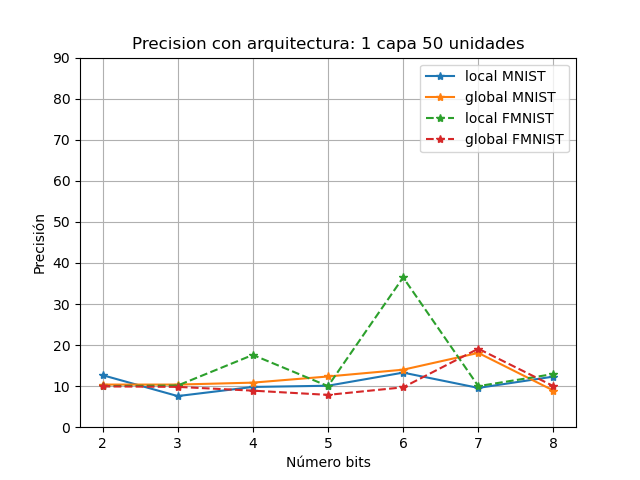
\includegraphics[width=\textwidth]{imagenes/dni/Precision con arquitectura: 1 capa 50 unidades.png}
    \end{subfigure}
    \begin{subfigure}[H]{0.45\textwidth}
    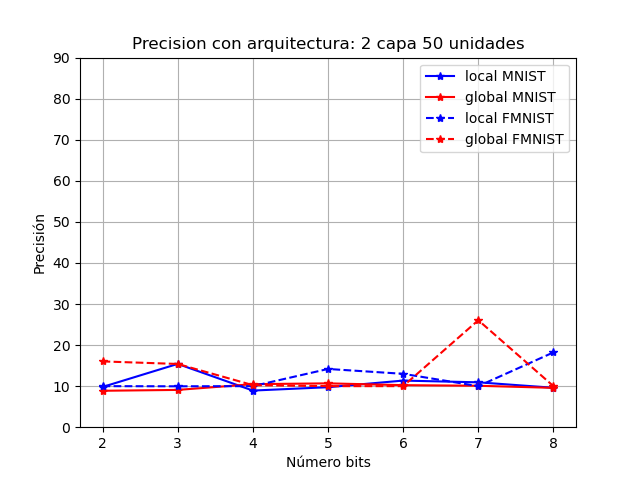
\includegraphics[width=\textwidth]{imagenes/dni/Precision con arquitectura: 2 capa 50 unidades.png}
    \end{subfigure}
    \begin{subfigure}[H]{0.45\textwidth}
    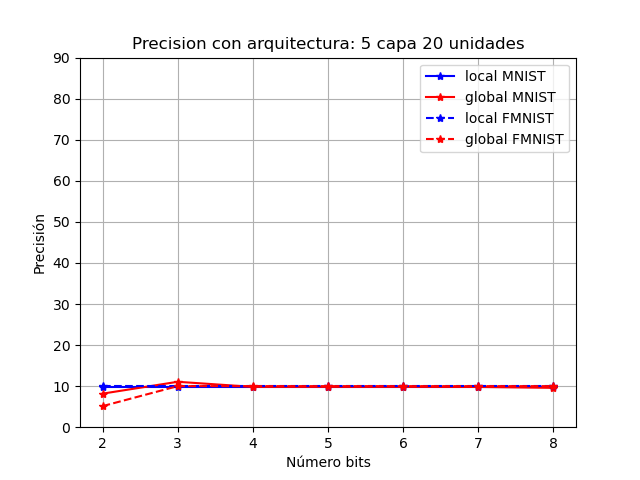
\includegraphics[width=\textwidth]{imagenes/dni/Precision con arquitectura: 5 capa 20 unidades.png} 
    \end{subfigure}
\end{figure}